\documentclass[10pt]{article}
\usepackage[utf8]{inputenc}
\usepackage[T1]{fontenc}
\usepackage{microtype}
\usepackage[margin=1in, left=1.25in, right=1.25in, top=1in, bottom=1in]{geometry}
\usepackage{algorithm}
\usepackage{algorithmic}
\usepackage{xurl}
\usepackage[numbers,square,sort&compress]{natbib}
\let\cite\citep
\usepackage[linktoc=all, bookmarksdepth=3, pdfstartview=FitH]{hyperref}
\hypersetup{colorlinks=true, linkcolor=blue, citecolor=blue, urlcolor=blue}
\urlstyle{same}
\usepackage{amsmath}
\usepackage{mathtools}
\usepackage{amsfonts}
\usepackage{amssymb}
\usepackage{bbold}
\usepackage{graphicx}
\usepackage{float}
\usepackage{placeins}
\setcounter{topnumber}{3}
\renewcommand{\topfraction}{0.90}
\renewcommand{\textfraction}{0.08}
\renewcommand{\floatpagefraction}{0.75}
\usepackage{caption}
\captionsetup[figure]{name=Fig.,labelfont=bf,labelsep=space}
\usepackage{booktabs}
\usepackage{multirow}
\usepackage{array}
\usepackage{tabularx}
\usepackage{longtable}
\usepackage{seqsplit}
\usepackage[normalem]{ulem}
\usepackage{amsthm}
\usepackage{enumitem}
\newtheorem{theorem}{Theorem}[section]
\newtheorem{lemma}[theorem]{Lemma}
\newtheorem{definition}[theorem]{Definition}
\newtheorem{corollary}[theorem]{Corollary}
\newtheorem{proposition}[theorem]{Proposition}
\newtheorem{remark}[theorem]{Remark}
\newtheorem{assumption}[theorem]{Assumption}
\newtheorem{example}[theorem]{Example}
\setlength{\emergencystretch}{2em}
\allowdisplaybreaks[2]
\DeclareRobustCommand{\lean}[1]{\nolinkurl{#1}}
\newcommand{\bamorv}{BAMOR}

\graphicspath{ {./} }

\newcommand{\BAMORArticleTitle}{Preference-Aligned Utility and Pareto Coverage in Non-Stationary Multi-Objective Reinforcement Learning}

\title{\BAMORArticleTitle}
\author{}
\date{}
\hypersetup{pdftitle={\BAMORArticleTitle},pdfauthor={}}

\begin{document}
\maketitle


\begin{abstract}
Pareto hypervolume measures the coverage of a policy's return set. In
preference-conditioned control, a separate question is how much utility the
policy delivers at the requested preference. We study both outcomes in custom
piecewise-stationary locomotion tasks using BAMOR, a context-conditioned
actor--critic that allocates training blocks across preference samplers and
update configurations. In a prespecified 20-seed comparison at 75,000
interactions, BAMOR's mean requested-preference utility exceeded that of
concave-augmented Pareto Q-learning (CAPQL) by 55.0\% on HalfCheetah and 6.0\%
on Hopper. Both primary confidence intervals included zero. Mean final-policy
hypervolume was lower on both tasks.

A retrospective baseline extension changed only CAPQL's training sampler.
Uniform full-simplex sampling raised its mean utility on HalfCheetah by 47.6\%
and lowered it on Hopper by 14.2\%. Against this variant, BAMOR's utility
difference on HalfCheetah remained uncertain. On Hopper, the interval for
BAMOR's 23.5\% mean advantage excluded zero in the retrospective comparison.
In separate experiments, retaining 19 snapshots increased observed coverage
over the included final actor on all 25 seeds. Progress-score ablations gave
mixed results. On Ant, disabling candidate searches partially recovered
mixed-preference utility under score-neutral allocation, and a gap to CAPQL
remained. Lean verifies a vector-target reselection example and a sufficient
score margin for local stability of matched candidates. Together these
results characterize sampler sensitivity, preference execution and archive
coverage under a fixed interaction budget.
\end{abstract}

\noindent\textbf{Keywords:} multi-objective reinforcement learning; non-stationary continuous control; preference-aligned execution; update portfolio; preference sampling; formal verification.


% ════════════════════════════════════════════════════════════════════════════
\section{Introduction}
% ════════════════════════════════════════════════════════════════════════════

Multi-objective reinforcement learning (MORL) seeks policies that trade off
conflicting reward coordinates across user preferences~\cite{Hayes2022MORL}.
In standard MORL benchmarks, performance is predominantly summarized by the
hypervolume (HV) of evaluated return vectors. For a single preference-conditioned
controller deployed online, however, set-level coverage and preference-aligned
execution are fundamentally distinct objectives: HV credits any non-dominated
return vector regardless of whether it was produced at the preference weight
that requested it, whereas operational deployment requires accurate scalarized
utility at the commanded weight itself.

This distinction becomes especially consequential in sample-constrained,
piecewise-stationary continuous control, where unobserved shifts in physical
parameters and objective saturation alter both reachable return geometries and
the effectiveness of training updates. A fixed interaction budget makes the
choice of training preferences consequential. A cone around equal weights,
as used in the CAPQL experiments~\cite{Lu2023CAPQL}, concentrates samples near
the center. A uniform simplex sampler extends support toward the boundary.
We test how this change affects direct utility under a common evaluation grid
on two tasks with different dynamics and reward coordinates. Adaptive operator
selection and curriculum allocation have been studied in evolutionary
optimization and multi-task learning~\cite{DaCosta2008AOS,Graves2017Curriculum},
and provide context for combining preference sampling, replay relabeling and
candidate action search in a shared MORL actor--critic.

We address these challenges through BAMOR, a context-conditioned update
portfolio framework coupled with a decoupled evaluation and diagnostic study.
At the transition level, BAMOR conditions a shared policy and twin vector
critics on observed dynamics via reward exponential averages, a lightweight
local action-response probe and a temporal-contrastive transition latent,
requiring no ground-truth regime labels. At the 1,500-step block level, a
portfolio allocates updates among coverage, recovery and extreme-preference
families. The selector corrects family allocation deficits and uses bounded,
scale-normalized reward changes estimated from training transitions. An
optional actor archive is retained passively to separate multi-policy Pareto
coverage from single-policy preference execution.

The main contributions of this work are threefold:
\begin{enumerate}
    \item \textbf{Context-conditioned quota-regulated MORL portfolio.} We formulate an integrated architecture combining label-free transition-context encoding, shared vector actor--critic training, and quota-regulated block allocation across preference-sampling, relabeling and candidate-search configurations, cleanly separating single-actor preference execution from multi-snapshot archive coverage.
    \item \textbf{Paired evaluation of utility, coverage and sampler sensitivity.} A prespecified CAPQL comparison and a retrospective sampler-only extension distinguish requested-preference utility from return-set coverage under equal interaction budgets. Separate archive, routing and Ant experiments characterize where gains depend on the evaluation object or training configuration.
    \item \textbf{Local target stability and archive properties.} A reselection example shows how an arbitrarily small scalar-score change can produce an order-one vector-target jump. Lean~4 verifies a fixed numerical instance, a strict score-margin certificate for local target stability, and conditional tracking and archive bounds.
\end{enumerate}

\section{Related Work}
% ════════════════════════════════════════════════════════════════════════════

\subsection{Preference-conditioned multi-objective reinforcement learning}
Envelope Q-learning~\cite{Yang2019Envelope} generalizes Bellman backups over
preference weights through convex-envelope maximization, and GPI-LS~\cite{Alegre2023GPILS}
couples generalized policy improvement with linear-support weight selection.
CAPQL~\cite{Lu2023CAPQL} introduces concave-augmented Pareto Q-learning with
entropy regularization on preference-conditioned vector critics, training
within a narrow angular cone around equal weights in its reported experiments.
CAPQL already evaluates scalarized returns at sampled preferences. Our
comparison pairs that type of execution measure with return-set coverage
on a common locked-mode grid. Hindsight Preference
Replay (HPR)~\cite{Shianifar2026HPR} augments off-policy replay via
return-aligned or neighborhood weight relabeling while keeping CAPQL's fixed
network and update rule. Rather than relying on a single static sampler or
relabeling heuristic, BAMOR coordinates heterogeneous sampling, relabeling,
candidate-ranking and regularization configurations over a context-conditioned
backbone, and explicitly contrasts requested-preference execution against
Pareto set hypervolume. Robust policy bootstrapping~\cite{Abdelfattah2023Bootstrapping}
maintains steppingstone policies to warm-start optimization after regime
changes; BAMOR's optional snapshot archive instead serves purely as a coverage
output without altering online controller training.

\subsection{Portfolio allocation and dynamic algorithm configuration}
Adaptive operator selection separates operator credit estimation from selection
probabilities using smoothed feedback and minimum probability floors~\cite{DaCosta2008AOS},
while automated curricula allocate training effort via learning-progress
signals~\cite{Graves2017Curriculum}. In reinforcement learning, online algorithm
selection~\cite{Laroche2018Selection} chooses among separate off-policy learners
sharing a replay buffer, whereas dynamic algorithm configuration (DAC) trains
meta-policies across problem instances~\cite{Biedenkapp2020DAC}, including
multi-agent hyperparameter control in evolutionary multi-objective
optimization~\cite{Xue2022MADAC}. Under tight single-run interaction budgets
where meta-training across instances is infeasible, BAMOR regulates a shared
actor--critic via deterministic family quota floors combined with zero-rollout
reward-coordinate progress routing.

\subsection{Non-stationary and robust continuous control}
Piecewise-stationary MDPs~\cite{Padakandla2020Survey,Lecarpentier2019NonStationary}
model abrupt environmental shifts between latent regimes. Contextual
MORL~\cite{Teoh2025MOCMDP} examines generalization across parameterized
multi-objective tasks, and robust MDPs~\cite{Wiesemann2013RobustMDP} optimize
worst-case returns over ambiguity sets. BAPR (preprint, arXiv:2605.16170)
combines change-point beliefs and context-conditioned Soft Actor-Critic
(SAC)~\cite{Haarnoja2018SAC} for single-objective piecewise-stationary
control. BAMOR extends the transition-context approach to vector rewards
and preference-conditioned policies. It replaces explicit change-point
beliefs with label-free context and allocates training across a portfolio
of update configurations.


% ════════════════════════════════════════════════════════════════════════════
\section{Problem and Evaluation Object}
\label{sec:problem_v23}

An unobserved mode $h_t$ determines the transition kernel and vector reward
$\mathbf r_t\in\mathbb R^m$. Modes change at unknown times. The learner observes
states, actions and rewards, and receives a preference $w\in\Delta^{m-1}$.
Training uses discounted scalar utilities $w^\top\mathbf Q$ with $\gamma=0.99$.
The primary evaluation object is the final preference-conditioned policy,
which computes context from its own observed transition history. This policy
is history-dependent through its context even though its actor parameters are
fixed at evaluation. A retained set $A$ of such policies defines a separate
archive-coverage outcome.

For a locked mode $h$, let
$J_h(\pi,w)=\mathbb E[\sum_{t=0}^{L-1}\mathbf r_t]$, where an episode ends on
termination or at $L\leq1000$ steps. These reported returns are undiscounted.
For the fixed evaluation grid $W$, the empirical candidate set is
$F_h(A)=\{\widehat J_h(\pi,w):\pi\in A,w\in W\}$, using three episodes per
candidate. We compute $\mathrm{HV}_r(F_h(A))$ with a fixed reference $r$ and
summarize environments by $H^{-1}\sum_h\mathrm{HV}_r(F_h(A))$. Mode-conditioned
fronts are not pooled into a cross-mode Pareto front. In archive experiments,
the final-actor subset and full archive are evaluated from the same rollouts.

The primary outcome in the twenty-seed study is same-preference final-policy utility,
\begin{equation}
 U(\pi)=\frac{1}{H|W|}\sum_{h=1}^H\sum_{w\in W}
              w^\top\widehat J_h(\pi,w).
 \label{eq:direct_utility}
\end{equation}
Here the sum runs over all modes and grid weights; there is no maximization
over other preferences or archived actors. A policy-set HV gain need not
increase this deployment-oriented outcome.

\paragraph{Why utility and coverage differ.}
Consider one mode and two requested weights $e_1=(1,0)$ and $e_2=(0,1)$.
A policy returning $(2,1)$ at $e_1$ and $(1,2)$ at $e_2$ has direct utility
$2$. A second policy that swaps these two responses has direct utility $1$.
Their return sets, and hence HV at any common reference, are identical.
This illustrative example separates preference-conditioned execution from
set coverage without assuming either metric determines the other.

\section{BAMOR Update Portfolio}
\label{sec:method_v23}

BAMOR denotes the frozen v25 implementation throughout the current comparisons.
At each interaction it constructs context from past transitions and conditions
one shared actor and twin vector critics on that context and a preference.
At each block boundary it chooses a fixed update configuration from a portfolio.
The configuration governs both collected preferences and replay updates for
the block; it does not instantiate a separate actor. Training rewards update
the selector, while test returns and mode identities are reserved for
evaluation. Algorithm~\ref{alg:bamor} gives the complete sequence.

\subsection{Context and replay}

One actor $\pi_\theta(a\mid s,w,z)$ and twin vector critics
$\mathbf Q_{\phi_i}(s,a,w,z)$ share a history-derived context $z$: reward
exponential averages, a scalar coordinate-response statistic and an
eight-dimensional learned transition embedding. The encoder reconstructs
scaled rewards and state displacements with temporal contrastive regularization.
Replay stores the collected context; preference relabeling changes only its
weight coordinates, not its stored history features. Mode labels are not
inputs. Appendix~\ref{app:implementation_details} specifies the coordinate
feature, encoder loss and exponential averages.

\subsection{Update configurations}
\label{sec:operator_portfolio}

Each arm $o$ specifies a preference sampler, relabel rate and copy count $C_o$,
critic candidate count $K_o^Q$, actor candidate count $K_o^\pi$, vector-loss
coefficient $\lambda_o$, and behavior-cloning coefficient $b_o$. There are seven
coverage arms, seven recovery arms and four extreme-preference arms, comprising
14 distinct sampler/update settings. Identical settings in different arm slots
retain separate scores and allocation counts. Relabeling
reuses vector-reward transitions under new preference inputs. All arms update
the same networks; the family names describe their intended roles. The full
configuration and warmup sequence are in Appendix~\ref{app:v23_operators}.

\paragraph{Critic update.}
For each replay transition, let $u$ denote its update preference after relabeling.
Set candidate preference $v_1=u$ and sample the remaining preferences using the
arm's replay sampler. Draw $a'_j\sim\pi_\theta(\cdot\mid s',v_j,z')$ and define
\begin{align}
 \mathbf q'_j&=\min_{i=1,2}\mathbf Q_{\phi_i^-}(s',a'_j,v_j,z'), \nonumber\\
 j^*&=\arg\max_j\{u^\top\mathbf q'_j-\alpha\log\pi_\theta(a'_j\mid s',v_j,z')\},\nonumber\\
 \mathbf y_v&=\mathbf r+\gamma(1-d_{\mathrm{term}})
       [\mathbf q'_{j^*}-\alpha\log\pi_\theta(a'_{j^*}\mid s',v_{j^*},z')\mathbf 1],\nonumber\\
 y_s&=u^\top\mathbf y_v.
 \label{eq:v25_targets}
\end{align}
Here the minimum is componentwise, targets are detached, $\alpha=0.2$ is fixed,
and only true termination sets $d_{\mathrm{term}}=1$; time limits retain the
bootstrap. The critic loss is
\begin{equation}
 \mathcal L_Q=\mathbb E\sum_{i=1}^2\left[
 (u^\top\mathbf Q_{\phi_i}(s,a,u,z)-y_s)^2+
 \frac{\lambda_o}{m}\|\mathbf Q_{\phi_i}(s,a,u,z)-\mathbf y_v\|_2^2\right].
 \label{eq:v23_critic_loss}
\end{equation}
Both target terms include the same selected-candidate entropy bonus.

\paragraph{Actor update.}
Generate $K_o^\pi$ actions $a_j\sim\pi_\theta(\cdot\mid s,v_j,z)$ with $v_1=u$.
Unlike the critic target above, rank these actions with critics conditioned on
the update preference $u$:
\begin{align}
 \mathbf q_j&=\min_{i=1,2}\mathbf Q_{\phi_i}(s,a_j,u,z),
 &j^\dagger&=\arg\max_j u^\top\mathbf q_j,\\
 \mathcal L_\pi&=\mathbb E\left[
 \alpha\log\pi_\theta(a_{j^\dagger}\mid s,v_{j^\dagger},z)
 -u^\top\mathbf q_{j^\dagger}
 +\frac{b_o}{d_a}\|a_{j^\dagger}-a\|_2^2\right].
 \label{eq:v23_actor_loss}
\end{align}
The discrete ranking is detached; gradients flow through the selected sampled
action and its generating policy log probability. $d_a$ is action dimension and
$a$ in the last term is the replay action. Thus multi-candidate updates are
specified training heuristics, not an exact optimality operator.

\subsection{Progress-driven block allocation}
\label{sec:method_v25}

Progress is measured in reward coordinates without multiplying by each
transition's collection preference. The first 5,000 transitions initialize
causal reward moments. Before each subsequent 1,500-transition block $k$, freeze
the per-objective standard deviations $s_{k,j}$ from past rewards. For the
first- and second-half means, the selected arm receives
\begin{equation}
 P_k=\frac{1}{m}\sum_{j=1}^m\tanh\left(
 \frac{\overline r^{(2)}_{k,j}-\overline r^{(1)}_{k,j}}{s_{k,j}}\right),
 \qquad q_o\leftarrow0.87q_o+0.13P_k,
 \label{eq:v25_progress}
\end{equation}
The arm stays fixed within a block, while interaction preferences change at
each transition. A completed block updates its score after the last reward
and before that transition's gradient; incomplete blocks remain unscored.
After ten prescribed warmup blocks, the selector first corrects family
allocation deficits against fractions $(0.36,0.22,0.18)$. Otherwise it samples
a family using the mean of its two highest arm scores, then an arm using its
own score, with softmax and uniform exploration at both levels. The score-blind
control substitutes zero routing scores while computing the same observations.
Exact temperatures, scales and scheduling parameters are in
Appendix~\ref{app:implementation_details}.

\subsection{Implementation budget and optional archive}

The main protocol uses 75,000 interactions and evaluates only the final actor
with its final encoder, without intermediate evaluation or actor selection.
Training context trackers persist across resets; evaluation initializes them
afresh. The separate 50k protocol retains 19 actors at steps
$5{,}000,7{,}500,\ldots,50{,}000$, all evaluated with the final encoder.
Archive evaluation does not feed the selector. Per-run network, optimization
and candidate resources are in Table~\ref{tab:v23_budget}.

\begin{algorithm}[t]
\caption{BAMOR-v25 training with optional actor retention}
\label{alg:bamor}
\label{sec:algorithm}
\begin{algorithmic}
\STATE Initialize networks, replay, context trackers and arm scores $q_o=0$; set $L=5{,}000$
\FOR{$t=1,\ldots,T$}
 \IF{$t\leq L$}
  \STATE Use the first warmup arm
 \ELSIF{a new scored block starts}
  \STATE Select an arm by Section~\ref{sec:method_v25}; freeze scales from past rewards
 \ENDIF
 \STATE Sample the arm's interaction preference; construct context from past transitions
 \STATE Act randomly if $t<L$, otherwise use the actor; observe the transition
 \STATE Update reward moments; for $t>L$, accumulate half-block rewards and allocation counts
 \IF{the 1,500-transition scored block is complete}
  \STATE Update $q_o$ by Eq.~\eqref{eq:v25_progress}, increment its block count and close the block
 \ENDIF
 \STATE Update context trackers; store the transition, both contexts and true-termination mask
 \IF{$t\geq L$}
  \STATE Relabel and expand a replay minibatch according to the selected arm
  \STATE Update critics using Eq.~\eqref{eq:v25_targets}, actor and target critics; update encoder
 \ENDIF
 \STATE Retain actor parameters at the prescribed steps, if an archive is requested
\ENDFOR
\STATE Leave any incomplete block unscored; evaluate the final actor in each locked mode
\STATE For archive experiments, also evaluate saved actors with the final encoder
\end{algorithmic}
\end{algorithm}

\FloatBarrier
\section{Supporting Mathematical Properties}

\paragraph{Target consistency and feedback.}
Simplex weights project the soft vector target exactly onto its scalar target
in Eq.~\eqref{eq:v25_targets} (Proposition~\ref{prop:soft_projection}). The
progress statistic and its score EMA stay in $[-1,1]$, and constant reward
offsets cancel at fixed scale (Proposition~\ref{prop:progress}). These are
properties of the implemented quantities.

\paragraph{Candidate selection and local stability.}
At equal weights, perturbing $(1,0),(0,0.9)$ to $(1,0),(0,1.1)$ changes the
unique selected vector's first coordinate by $1$ despite an input change of
only $0.2$ (Proposition~\ref{prop:reselection}). Scalar-maximization stability
therefore does not imply selected-vector stability. For matched actions and
contexts, let $S_j=u^\top q_j+e_j$, with critic-coordinate perturbations at
most $\epsilon\geq0$ and entropy-bonus perturbations at most $\rho\geq0$. If the winner
$j^*$ satisfies
\begin{equation}
 S_{j^*}-S_j>2\delta\quad(j\neq j^*),\qquad\delta=\epsilon+\rho,
 \label{eq:main_candidate_margin}
\end{equation}
the winner is unchanged. With fixed reward and bootstrap multiplier $b\geq0$,
the soft targets obey $\|Y-\widetilde Y\|_\infty\leq b\delta$
(Proposition~\ref{prop:candidate_margin}).

Appendix~\ref{sec:theory} gives the Lean proofs and conditional tracking and
archive results. Tracking requires contractive selected maps, bounded update
error and bounded selected-map residual. HV monotonicity fixes returns,
reference and encoder; archive selection additionally requires uniform return
accuracy. These assumptions delimit the supporting analysis.


\paragraph{Use of generative AI.}
Google Gemini assisted with manuscript restructuring and presentation.
OpenAI Codex assisted with manuscript revision, statistical cross-checks and
preparation of the reproducibility materials.

\section{Experiments}
\label{sec:experiments}
% ════════════════════════════════════════════════════════════════════════════

\subsection{Evaluation design}
\label{sec:mujoco_3d}

The primary comparison evaluated unchanged BAMOR-v25 and fully seeded CAPQL
at 75k interactions on HalfCheetah and Hopper, using seeds 1601--1620 and only
the final actor. An earlier five-seed pilot motivated the task selection and
utility hypothesis; confirmation seeds and analysis were fixed before training.
The cohorts remain separate (Appendix~\ref{app:experiment_details}).

The custom piecewise-stationary tasks have two objectives/four modes on
HalfCheetah, three/four on Hopper and three/three on Ant. Modes alter physics
and reward scales or smooth caps; exponential dwell lengths have scale 25k
and minimum 1,000. Evaluation locks each mode, uses deterministic actions at
21 full-simplex weights with three paired reset seeds, and ends on termination
or at 1,000 steps. Training schedules and evaluation inputs are paired;
mode-wise fronts are not pooled (Appendix~\ref{app:task_details}).

Direct utility $U$ evaluates the requested preference; final HV evaluates the
final actor's return set; archive HV evaluates retained actors. W/L/T denotes
paired seed wins/losses/ties, including every pair. Relative differences compare
cohort means; utilities and raw HV are not pooled across tasks. BAMOR uses width
64 and CAPQL width 256, with equal interaction budgets but different update
computation (Table~\ref{tab:v23_budget}).

\subsection{Twenty-seed final-policy utility}
\label{sec:utility_confirmation}

BAMOR achieved higher observed mean direct utility on both tasks
(Table~\ref{tab:utility_confirmation}). HalfCheetah means were 296.32 versus
191.17 for CAPQL, a difference of 105.15 (+55.00\%); Hopper means were 436.59
versus 411.93, a difference of 24.67 (+5.99\%). Each task had 13 positive
and seven negative seed-paired differences. Every run used the original
method settings, with no intermediate evaluation or checkpoint selection.

% Generated by make_evidence_tables.py from completed readouts.
\begin{table}[t]
\centering\small
\caption{Final-policy direct utility at 75k training interactions, 20 independent seed pairs per environment (1601--1620). Means are BAMOR / CAPQL; $\Delta U$ and its interval are in utility units. The paired 97.5\% bootstrap intervals implement the prespecified two-environment criterion. W/L/T includes every seed pair.}
\label{tab:utility_confirmation}
\begin{tabular}{@{}lrrrrr@{}}
\toprule
Environment & $U$: BAMOR / CAPQL & $\Delta U$ & Relative & 97.5\% CI & W/L/T \\
\midrule
HalfCheetah & 296.32 / 191.17 & +105.15 & +55.00\% & $[-33.80,\ 235.83]$ & 13/7/0 \\
Hopper & 436.59 / 411.93 & +24.67 & +5.99\% & $[-58.64,\ 105.58]$ & 13/7/0 \\
\bottomrule
\end{tabular}
\end{table}


\paragraph{Prespecified uncertainty analysis.}
Intervals used 20,000 bootstrap resamples of complete training-seed pairs,
retaining their mode and preference outcomes together. The frozen criterion
used a 97.5\% percentile interval per task for nominal 95\% Bonferroni family
coverage; bootstrap coverage is approximate. Both intervals included zero, as
did ordinary 95\% intervals (Appendix~\ref{app:experiment_details}). The
observed means therefore did not meet the criterion for an expected-utility
advantage. No pairs were excluded and no pilot seeds were added.

\paragraph{Coverage and computational cost.}
Final HV and runtime gave different orderings from mean utility
(Table~\ref{tab:utility_secondary}). BAMOR's mean final HV was 4.84\% lower
on HalfCheetah and 5.77\% lower on Hopper, with 10 and eight wins out of 20,
respectively. The descriptive paired HV intervals included zero. Mean
training time was 1.67 and 1.73 times CAPQL's. These are measured times on a
shared cluster, not dedicated-machine benchmarks; both methods used two CPU
threads per run.

% Generated by make_evidence_tables.py from completed readouts.
\begin{table}[t]
\centering\small
\caption{Secondary outcomes on the same 20-seed cohorts as Table~\ref{tab:utility_confirmation}. HV is the relative difference of final-policy means. Times are mean seconds per run, BAMOR / CAPQL, on the shared CPU cluster with two threads per run.}
\label{tab:utility_secondary}
\begin{tabular}{@{}lrrrr@{}}
\toprule
Environment & Final HV & W/L/T & Training (s) & Evaluation (s) \\
\midrule
HalfCheetah & -4.84\% & 10/10/0 & 1635.8 / 981.5 & 152.5 / 81.8 \\
Hopper & -5.77\% & 8/12/0 & 1759.7 / 1016.8 & 122.6 / 69.1 \\
\bottomrule
\end{tabular}
\end{table}


The 80 runs consumed 6,000,000 training and 16,512,980 evaluation interactions.
Evaluation did not enter replay or selector feedback. Initialization probes,
prelaunch tests and per-cohort costs are accounted for in
Appendix~\ref{app:experiment_details}.

\subsection{Archive coverage and feedback attribution}

At 50k interactions, both methods retained 19 actors. This retrospective
comparison used 15 HalfCheetah and five Hopper/Ant seeds, adding CAPQL after
the BAMOR cohort was inspected. Archive coverage favored BAMOR most strongly
on Hopper, with five paired wins (Table~\ref{tab:matched_archive}). Ant final
HV fell on all five seeds; HalfCheetah's 16.21\% archive-mean gain accompanied
only 0.74\% in final HV. The early CAPQL cohort's incomplete RNG seeding is
documented in Section~\ref{sec:limits}.

% Generated by make_evidence_tables.py from completed readouts.
\begin{table}[t]
\centering\small
\caption{Retrospective 50k comparison: v25 minus CAPQL, with 19 actors in each archive. Percentages compare cohort means; W/L/T denotes paired seed wins/losses/ties. The early CAPQL runs omitted two RNG seeds (Section~\ref{sec:limits}).}
\label{tab:matched_archive}
\begin{tabular}{lrrrrr}
\toprule
Environment & $n$ & Archive HV & W/L/T & Final HV & W/L/T \\
\midrule
HalfCheetah & 15 & +16.21\% & 10/5/0 & +0.74\% & 8/7/0 \\
Hopper & 5 & +140.39\% & 5/0/0 & +58.67\% & 3/2/0 \\
Ant & 5 & +1.17\% & 3/2/0 & -11.07\% & 0/5/0 \\
\bottomrule
\end{tabular}
\end{table}


The score-blind control retained networks, arms, family floors and archive
schedule while replacing routing scores with zero
(Table~\ref{tab:selector_effect}). Adaptive selection did not improve mean
archive or final HV on HalfCheetah or Ant. Hopper's positive means had two
wins, one loss and two ties; seven of fifteen HalfCheetah pairs tied exactly.
These observations separate an external archive advantage from evidence of a
consistent feedback benefit.

% Generated by make_evidence_tables.py from completed readouts.
\begin{table}[t]
\centering\small
\caption{Feedback attribution at 50k: unchanged v25 adaptive minus its score-blind control on the same cohorts as Table~\ref{tab:matched_archive}.}
\label{tab:selector_effect}
\begin{tabular}{lrrrrr}
\toprule
Environment & $n$ & Archive HV & W/L/T & Final HV & W/L/T \\
\midrule
HalfCheetah & 15 & -0.15\% & 3/5/7 & -0.85\% & 4/4/7 \\
Hopper & 5 & +6.54\% & 2/1/2 & +59.56\% & 2/1/2 \\
Ant & 5 & -1.00\% & 1/3/1 & -3.33\% & 0/4/1 \\
\bottomrule
\end{tabular}
\end{table}


\subsection{Ant mixed-preference diagnosis}
\label{sec:ant_diagnosis}

The earlier fully seeded 75k pilot lost all five Ant pairs in utility and final
HV: mean utility was 988.8 versus CAPQL's 1364.9, and mean final HV was 6.94\%
lower (Table~\ref{tab:final_policy}). Failure was concentrated in mixed weights
containing the energy objective. On that inspected cohort, re-scalarizing evaluated
returns showed that v25's pure-energy policy beat its corresponding
mixed-preference policy at 66 of 70 mode-0 seed--weight cells. This comparison
uses the same saved actor and requires no extra environment interactions.

Candidate-search ablations and an independent structure-by-selector pilot did
not close the CAPQL gap. The latter's primary residual effect had only two of
five wins, and its residual adaptive arm still trailed CAPQL by 247.9 mixed
utility and 2.06\% final HV (Appendix~\ref{app:ant_diagnostics}). The residual
variant was not adopted; cross-environment BAMOR remains unchanged v25.


\section{Discussion}
\label{sec:discussion}

\paragraph{Execution, coverage and sampler sensitivity.}
A return set can have high hypervolume even when its behaviors are poorly
matched to the preferences that request them (Section~\ref{sec:problem}).
The sampler-only contrast in CAPQL changes observed mean utility by
$+47.61\%$ on HalfCheetah and $-14.20\%$ on Hopper. The two tasks differ in
physics, reward coordinates and objective count, so the experiment does not
identify the role of dimension alone. BAMOR uses the same portfolio design
on both tasks, with the highest observed mean utility among the three tested
configurations.

\paragraph{Snapshot retention and training choices.}
Retention increases the number of evaluated candidates. The archive gains
measure this increase in coverage for one training method. Using the archive
to fulfill a particular preference requires a policy-selection rule and
separate evaluation. The score-neutral comparison keeps the family quota
mechanism in both arms, and the observed routing effects vary by task.
Ant exhibits a large difference between querying the actor at a mixed weight
and applying a vertex behavior to that query. The own-preference ablations
show that candidate search contributes to the observed deficit under some
settings. Attribution to gradient routing, target bias or simplex sampling
would require interventions that vary these mechanisms separately.

\subsection{Limitations}
The primary comparison used independent seeds, with tasks and the utility
hypothesis motivated by a pilot. The sampler extension reused the inspected
cohort. The main runs match interactions, while BAMOR uses a 64-width
context-conditioned network and more candidate evaluations than 256-width
memoryless CAPQL. HPR and GPI-LS were not evaluated. A common backbone and a
score-neutral control at 75k on both primary tasks would help separate
representation, update configuration and routing effects.

Only two of the 20 training histories per main task visited all four modes.
Evaluation holds each mode fixed and uses three resets per preference.
Switch-aligned recovery, learning curves across budgets and performance on
new task families remain open. The context includes an observation-coordinate
ratio specific to the implementation, and replay retains context generated
by earlier encoder parameters. Half-block reward differences can reflect
preference sampling, episode resets and mode changes as well as learning.
The Ant interventions use five development seeds, and the independent
residual-actor study has five seeds with a different design. The formal results
assume matched candidates for local stability, contraction and residual bounds
for tracking, or uniform return-estimation accuracy for archive selection.
Their assumptions have not been established along neural training.

\section{Conclusion}
On two piecewise-stationary locomotion tasks, BAMOR had higher observed mean
requested-preference utility and lower mean final-policy hypervolume than
native CAPQL at 75k interactions. Both primary utility contrasts remained
uncertain. Changing CAPQL's training sampler substantially altered the
HalfCheetah comparison, and the Hopper contrast with full-simplex CAPQL
remained positive under the follow-up's interval procedure. Separate results
show increased coverage from retaining checkpoints and partial recovery of
mixed-preference utility in Ant ablations. Together with the local
target-stability result, the experiments motivate reporting requested-preference
utility, return-set coverage and routing ablations separately.

\section*{Statements and Declarations}
\paragraph{Data and code availability.}
The simulation records supporting the reported results and the analysis and
training code are available in the supplementary material (Online Resource~1).
The archive contains compact seed-level records rather than raw trajectories
or model checkpoints.

\paragraph{Online Resource 1.}
Reproducibility archive (\texttt{ESM\_1.zip}): frozen protocols, compact
simulation records, analysis scripts, training code and Lean proof sources.

\bibliographystyle{unsrtnat}
\bibliography{refs}

\newpage
\appendix
\onecolumn
\section{Implementation-Facing Mathematical Properties}
\label{sec:theory}
\label{app:lean}

The statements below are formalized in \path{BAMOR/Implementation.lean},
namespace \path{BAMOR.Implementation}. They distinguish target construction,
feedback statistics, conditional tracking and archive evaluation. Algebra is
over exact real numbers. The Lean source and its imported auxiliary results
are replayed with Lean~4.28.0 and Mathlib~4.28.0.

\subsection{Soft targets and continuation masks}
\label{app:soft_target}

Let $u\in\Delta^{m-1}$, $b=\gamma(1-d_{\mathrm{term}})$ and
$e=-\alpha\log\pi_\theta(a'_{j^*}\mid s',v_{j^*},z')$.
For the selected vector $q$, define $Y_i=r_i+b(q_i+e)$.

\begin{proposition}[Consistent scalar projection]
\label{prop:soft_projection}
The v25 targets satisfy
\begin{equation}
 u^\top Y=u^\top r+b(u^\top q+e).
 \label{eq:soft_projection}
\end{equation}
At true termination $b=0$, $Y=r$. Replacing a continuing-task time-limit
mask $b=\gamma$ by zero removes $\gamma(q_i+e)$ from coordinate $i$.
\end{proposition}
\begin{proof}
Distribute the scalar product and use $\sum_i u_i=1$ for the common entropy
bonus. The mask identities follow by substitution. Lean:
\path{soft_target_projection}, \path{terminal_target}, and
\path{truncation_target_difference}.
\end{proof}

With the same selected candidate and entropy bonus in two targets,
$|q_i-\widetilde q_i|\leq\epsilon$ and $b\geq0$ give
$|Y_i-\widetilde Y_i|\leq b\epsilon$
(\path{frozen_target_lipschitz}). The qualification about selection matters.

\begin{proposition}[Candidate reselection can amplify vector differences]
\label{prop:reselection}
For $u=(1/2,1/2)$, consider candidates $(1,0),(0,0.9)$ and their perturbed
versions $(1,0),(0,1.1)$, with equal entropy bonuses. All candidate coordinates
change by at most $0.2$, but the first coordinate of the selected vector changes
by $1$. Both scalar maximizers are unique.
\end{proposition}
\begin{proof}
The scalar scores change from $(0.5,0.45)$ to $(0.5,0.55)$. The maximizing
candidate switches from the first to the second. The coordinatewise bound and
selected-vector difference are checked exactly by
\path{candidate_reselection_counterexample}; strict score inequalities are
checked by \path{candidate_reselection_unique}.
\end{proof}

Thus the scalar maximum's non-expansiveness cannot be transferred to its
selected vector. The counterexample also applies to equal twin critics and
fixed candidate actions; neither critic disagreement nor a tie is necessary.

\begin{proposition}[Margin-certified target stability]
\label{prop:candidate_margin}
Fix a nonempty finite set of candidate actions and their context inputs,
$u\in\Delta^{m-1}$, reward $r$ and bootstrap multiplier $b\geq0$.
For candidate $j$, let $q_j$ be the coordinatewise minimum of the two critic
vectors, $e_j$ its entropy bonus and $s_j=u^\top q_j+e_j$ its ranking score.
Compare these with perturbed values $\widetilde q_j,\widetilde e_j$ satisfying
\begin{equation}
 |q_{j,i}-\widetilde q_{j,i}|\leq\epsilon,\qquad
 |e_j-\widetilde e_j|\leq\rho,\qquad
 \delta=\epsilon+\rho,\quad \epsilon,\rho\geq0.
 \label{eq:candidate_perturbation}
\end{equation}
If $s_{j^*}-s_j>2\delta$ for every $j\neq j^*$, then $j^*$ is the unique
maximizer of both score sets. The corresponding soft targets satisfy
\begin{equation}
 |Y_i-\widetilde Y_i|\leq b\delta\quad\text{for every }i,
 \qquad
 |u^\top Y-u^\top\widetilde Y|\leq b\delta.
 \label{eq:margin_target_bound}
\end{equation}
\end{proposition}
\begin{proof}
The simplex conditions and the triangle inequality give
$|s_j-\widetilde s_j|\leq\epsilon+\rho=\delta$.
Hence $\widetilde s_{j^*}-\widetilde s_j
\geq s_{j^*}-s_j-2\delta>0$.
With the selected index unchanged, the coordinatewise target difference is
$b|(q_{j^*,i}-\widetilde q_{j^*,i})+(e_{j^*}-\widetilde e_{j^*})|
\leq b\delta$. Simplex projection gives the scalar bound.
Lean: \path{soft_score_perturbation},
\path{strict_margin_preserves_winner}, and
\path{margin_selected_target_lipschitz}.
\end{proof}

\subsection{Progress-score properties}
\label{app:progress}

For the first and second half-block reward means $a,b\in\mathbb R^m$ and
the frozen positive scale $s$, write
\begin{equation}
 P(a,b;s)=\frac{1}{m}\sum_i\tanh\frac{b_i-a_i}{s_i}.
\end{equation}

\begin{proposition}[Bounded, centered block feedback]
\label{prop:progress}
For $m\geq1$, $-1\leq P\leq1$. For any per-objective offset $c$,
$P(a+c,b+c;s)=P(a,b;s)$. Positive rescaling preserves the score if the
supplied scales are rescaled by the same coordinatewise factors. If
$q,P\in[-1,1]$ and $\eta\in[0,1]$, then
$(1-\eta)q+\eta P\in[-1,1]$.
\end{proposition}
\begin{proof}
Each hyperbolic tangent is in $(-1,1)$, so its finite average is in $[-1,1]$.
Offsets cancel in the difference, and common nonzero factors cancel in the
ratio. The score update is a convex combination. Lean:
\path{progress_score_bounds}, \path{progress_translation_invariant},
\path{progress_rescaling_invariant}, and \path{score_ema_bounds}.
\end{proof}

Starting at zero, v25's score EMA remains bounded by induction; unselected
arms and incomplete blocks leave scores unchanged. Its fixed $10^{-6}$ scale
floor means that rescaling invariance need not hold when clipping changes.
The propositions concern the statistic on supplied observations and scales,
not an invariant training trajectory. A reward increase caused by a mode
change enters the same numerator as an improvement caused by learning.

\subsection{Conditional tracking with update error}
\label{app:tracking_current}

Let $T_{n,o}$ be a family of maps on a metric space, $o_n$ the realized
selected arm and $q_n^*$ a reference trajectory. Assume, for all $n,o,x,y$,
\begin{align}
 d(T_{n,o}x,T_{n,o}y)&\leq\gamma d(x,y),\qquad 0\leq\gamma<1,\nonumber\\
 d(q_{n+1},T_{n,o_n}q_n)&\leq\epsilon,\nonumber\\
 d(T_{n,o_n}q_n^*,q_{n+1}^*)&\leq\Delta,
 \qquad \epsilon,\Delta\geq0.
 \label{eq:tracking_assumptions}
\end{align}
The last quantity includes the selected operator's mismatch with the reference,
not just physical environment drift.

\begin{proposition}[Approximate selected-map tracking]
\label{prop:tracking_current}
Under Eq.~\eqref{eq:tracking_assumptions}, for every $n\geq0$,
\begin{equation}
 d(q_n,q_n^*)\leq\gamma^n d(q_0,q_0^*)+
                    \frac{\epsilon+\Delta}{1-\gamma}.
\end{equation}
\end{proposition}
\begin{proof}
Two triangle inequalities yield
$d(q_{n+1},q_{n+1}^*)\leq\gamma d(q_n,q_n^*)+\epsilon+\Delta$.
Apply the geometric recurrence bound \path{BAMOR.anytime_tracking_bound}.
The full composition is \path{approximate_selected_tracking}.
\end{proof}

The residual term is an upper bound, not a lower error floor, and the initial
error term remains part of the bound. No comparison with CAPQL follows from
this recurrence alone.

The arm sequence may depend on observed history: the inequality compares two
inputs using the \emph{same} selected map at that step. It is not a comparison
between two feedback trajectories that can choose different arms. The finite
state/action auxiliary operator in \path{BAMOR.lean} uses per-objective action
maxima and frozen belief/penalty parameters. Its contraction theorem is valid
for that operator. Proposition~\ref{prop:reselection} shows why the vector
candidate update needs separate treatment.

\subsection{Continuous hypervolume and policy selection}
\label{app:archive_current}

Fix the mode, encoder, return vectors $J(p)$ and reference $r$. A candidate
$p$ denotes an actor/preference pair. For a finite archive $A$, define
\begin{equation}
 D_r(A)=\bigcup_{p\in A}[r,J(p)],\qquad
 \mathrm{HV}_r(A)=\operatorname{vol}_m(D_r(A)),
\end{equation}
where the interval is coordinatewise and is empty when any upper coordinate
is below the reference. This is the maximization convention.

\begin{proposition}[Continuous archive monotonicity]
\label{prop:hv_current}
The dominated region is compact and measurable with finite volume, and
$A\subseteq B$ implies
$D_r(A)\subseteq D_r(B)$ and $\mathrm{HV}_r(A)\leq\mathrm{HV}_r(B)$.
\end{proposition}
\begin{proof}
Each finite-coordinate rectangle is compact and measurable; the union is
finite, so its Lebesgue volume is finite. Every rectangle indexed by $A$ also
occurs in $B$, and Lebesgue measure is monotone. Lean:
\path{dominated_region_measurable}, \path{dominated_region_mono}, and
\path{hypervolume_mono}. The measure is initially valued in $[0,\infty]$;
\path{hypervolume_ne_top} proves finiteness, and
\path{hypervolume_toReal_mono} transfers monotonicity to the real-valued HV
used here. This concerns continuous volume rather than a grid-cell count.
\end{proof}

\begin{proposition}[From estimated archive scores to a selected policy]
\label{prop:selection_regret}
Fix a query and scalar scores $J,\widehat J$ on a nonempty finite archive $A$.
If $|\widehat J(p)-J(p)|\leq\epsilon$ for every $p\in A$ and
$\hat p\in\arg\max_{p\in A}\widehat J(p)$, then
\begin{equation}
 \max_{p\in A}J(p)-J(\hat p)\leq2\epsilon.
\end{equation}
\end{proposition}
\begin{proof}
For every $p\in A$,
$J(p)\leq\widehat J(p)+\epsilon\leq\widehat J(\hat p)+\epsilon
\leq J(\hat p)+2\epsilon$. Take the finite maximum. Lean:
\path{archive_selection_regret}.
\end{proof}

This is a conditional policy-selection bound, not regret of the training-arm
selector. It requires a uniform evaluation-error bound and an actual selection
rule. Archive HV supplies neither. The experiments report fixed-rollout archive
coverage and direct final-policy utility separately.

\subsection{Proof scope and retained auxiliary results}

The current results formalize target consistency, bounded score updates,
margin-certified target stability, conditional tracking and fixed-value archive
comparisons. The margin condition uses matched candidates and explicit bounds
on critic and entropy outputs; these bounds have not been established along
the training trajectories. Equality at the $2\delta$ threshold can produce a
tie, whereas failing the sufficient condition does not imply a switch.
The results do not prove
convergence of the implemented actor--critic or a causal improvement from its
progress selector. No uniform return-estimation error bound is established by
the three-reset evaluation protocol. Updating the encoder, re-estimating old
returns or replacing archive members changes the object in
Proposition~\ref{prop:hv_current}.

The earlier contraction, localized-drift, anchor and belief results remain in
\path{BAMOR.lean} and \path{RegimeBelief.lean}. Their definitions concern the
auxiliary frozen tabular model. Anchor concavity is with respect to the
preference, not actor parameters. \path{BAMOR-Counterproof.lean} retains its
Q-dependent-belief examples; its posterior-ratio threshold assumes a specific
power sequence, rather than deriving a BOCD detection rate. These results are
retained in the proof repository without duplicating their full historical
exposition in this appendix.

\subsection{Historical v23 target and score}
\label{app:v23_legacy}

The v23 critic used the episode-end mask $d$, including time limits, and
different scalar and vector targets:
\begin{equation}
 y_s=u^\top r+\gamma(1-d)(u^\top q+e),\qquad
 \mathbf y_v=r+\gamma(1-d)q.
\end{equation}
Hence $y_s-u^\top\mathbf y_v=\gamma(1-d)e$ for simplex weights. V24 repaired
both the mask and this target inconsistency; v25 retains those repairs.

For a 1,500-transition block, v23 used $g_t=w_t^\top r_t$ and
$R_k=\overline g_k-0.08\,\operatorname{std}(g_t)
-0.04(\overline g_k-\min_t g_t)$.
With $\delta_k=R_k-B$, its updates were $B\leftarrow0.9B+0.1R_k$,
$S\leftarrow0.9S+0.1|\delta_k|$, followed by
$q_o\leftarrow0.87q_o+0.13\tanh(\delta_k/\max(S,10^{-6}))$.
The first block initialized $B=R_k,S=1$ before these updates.
V25 replaces this score and starts its scored blocks after 5,000 transitions;
the operator configurations and family-allocation rule are unchanged.

\clearpage
\section{Context Probes, Preference Samplers and Resource Details}
\label{app:implementation_details}

Table~\ref{tab:v23_budget} gives the model, training and per-run resource settings.

\subsection{Transition-derived context and local action-response probe}

The label-free context vector $z_t$ concatenates squashed reward exponential
averages $\tanh(\overline{\mathbf{r}}/3)$ (EMA rate $0.2$), a scalar local
action-response probe, and an eight-dimensional transition latent $e_\psi$
(online EMA rate $0.35$). Using zero-based state and action indices, the local
action-response probe records the short-step gain ratio $v = s'_1 / a_0$
whenever $|a_0| > 0.05$, $v$ is finite and $|v| < 10$, updating a causal EMA
$\bar{v}$ at rate $0.2$ from the first accepted sample and outputting
$\operatorname{clip}((\bar{v} - 1)/0.5, -3, 3)$ (zero prior to first acceptance).
This lightweight probe provides a fast responsiveness summary alongside reward
statistics and learned transition embeddings without assuming parametric system
identification.

The transition encoder maps $(s, a, \tanh(\mathbf{r}/3), s' - s)$ to an
eight-dimensional $\tanh$-bounded latent. Its auxiliary objective minimizes
mean-squared reconstruction error on $\tanh(\mathbf{r}/3)$ and scaled state
displacement $\tanh((s' - s)/3)$, adds an $\ell_2$ latent penalty with weight
$10^{-4}$, and applies a temporal contrastive loss (weight $0.2$, temperature
$0.2$, positive time window $256$ steps). Replay transitions retain their
collected context features during preference relabeling; no regime labels enter
training or evaluation.

\subsection{Preference samplers}

Four preference-sampling rules parameterize the portfolio across $m$ objectives
(Table~\ref{tab:operators}):
\begin{itemize}[leftmargin=1.5em,itemsep=2pt,topsep=3pt]
 \item \texttt{uniform}: draws $w \sim \mathrm{Dir}(\mathbf{1}_m)$ independently
       during both environment interaction and replay relabeling/candidate
       generation.
 \item \texttt{edge}: uses the $(m+1)$-point corners-plus-center set
       $\mathcal{E}_m = \{e_1, \ldots, e_m, \frac{1}{m}\mathbf{1}_m\}$, cycling
       deterministically by $(t-1) \bmod (m+1)$ during interaction and sampling
       uniformly from $\mathcal{E}_m$ in replay.
 \item \texttt{stratified}: for $m = 2$ (HalfCheetah), uses the 11-point uniform
       simplex grid $\{(i/10, 1 - i/10) : i = 0, \ldots, 10\}$ (cyclic in
       interaction, uniform in replay). For $m \geq 3$ (Hopper and Ant),
       \texttt{stratified} uses the $(m+1)$-point corner-center set
       $\mathcal{E}_m$, so slots C5 and R2 coincide functionally with C4 on
       three-objective tasks (yielding 13 functionally distinct settings on
       $m = 3$, with zero discrete mass on non-vertex edges of the
       three-objective simplex).
 \item \texttt{mixed}: during interaction at step $t$, selects \texttt{edge}
       when $t \equiv 0 \pmod 3$ ($1/3$), \texttt{stratified} on remaining even
       steps ($1/3$), and $\mathrm{Dir}(\mathbf{1}_m)$ on remaining odd steps
       ($1/3$). Each branch occurs twice per six consecutive steps.
       For three objectives, the first two branches together assign two
       thirds of interaction requests to the corners-plus-center set.
       In replay, each draw independently selects
       $\mathrm{Dir}(\mathbf{1}_m)$ or \texttt{stratified} with probability
       $0.5$ each.
\end{itemize}

\subsection{Block allocation hyperparameters and per-run resources}

During the first $5{,}000$ transitions, the initial coverage slot supplies
preferences while causal per-objective reward means and variances initialize
(EMA rate $1/1500$). Before each subsequent $1{,}500$-step block, per-objective
standard deviations are frozen with numerical floor $10^{-6}$, and completed
blocks update the active slot score via $q_o \leftarrow 0.87\,q_o + 0.13\,P_k$
prior to that step's gradient update (incomplete terminal blocks remain
unscored). After ten deterministic warmup blocks
(Appendix~\ref{app:operators}), the selector enforces minimum family quota
fractions $(0.36, 0.22, 0.18)$ by choosing the family with the largest positive
deficit; otherwise it samples a family via a softmax over the mean of its two
highest slot scores (temperature $0.22$, uniform exploration mixture $0.16$)
and then samples a slot within that family (temperature $0.28$, exploration
mixture $0.16$). Within-family sampling still uses slot scores during family
deficit correction. The score-neutral control passes zero scores to routing
and keeps the quotas, warmup blocks and exploration mixtures.
At 75k interactions there are 46 complete feedback blocks: ten scheduled
warmup blocks and 36 subsequent blocks. The last 1,000 training steps use
a selected slot but provide no complete-block score.

\begin{table}[htbp]
\centering\small
\caption{Hyperparameters and per-run computational settings for the 75k
sample-constrained benchmark. Hidden widths apply to two-layer MLPs; the 50k
archive study uses identical network and optimizer settings while retaining 19
periodic actor snapshots.}
\label{tab:v23_budget}
\begin{tabular}{lcc}
\toprule
Quantity & BAMOR & CAPQL (Native / Full-Simplex)\\
\midrule
Training interactions & 75,000 & 75,000\\
Learning starts / replay minibatch & 5,000 / 256 & 5,000 / 256\\
Actor and critic hidden width & 64 & 256\\
Replay buffer capacity & 500,000 & 500,000\\
Learning rate / target Polyak rate & $3\times 10^{-4}$ / $0.005$ & $3\times 10^{-4}$ / $0.005$\\
Evaluated actors / preference grid $|W|$ & 1 / 21 & 1 / 21\\
Evaluation episodes per weight and mode & 3 & 3\\
Preference copies per update ($C_o$) & 1--3 & 1\\
Critic / actor candidates ($K_o^Q$ / $K_o^\pi$) & 1--5 / 1--5 & 1 / 1\\
Training preference distribution & 18-slot portfolio & $22.5^\circ$ cone / $\mathrm{Dir}(\mathbf{1})$\\
\bottomrule
\end{tabular}
\end{table}

\clearpage
\section{Portfolio Configuration Specification}
\label{app:operators}
\begin{table}[ht]
\centering\small
\caption{The 18 allocation slots of the BAMOR update portfolio across coverage
(C), recovery (R) and extreme-preference (E) families. Relabel denotes the
fraction of the replay minibatch assigned fresh preferences; $C_o$ counts total
preference copies per batch; $K_o^Q$ and $K_o^\pi$ are critic and actor
candidate counts; $\lambda_o$ and $b_o$ weight vector-target and
behavior-cloning losses.}
\label{tab:operators}
\begin{tabular}{llrrrrrr}
\toprule
Slot & Sampler & Relabel & $C_o$ & $K_o^Q$ & $K_o^\pi$ & $\lambda_o$ & $b_o$\\
\midrule
C1 & edge & 1 & 3 & 1 & 1 & 0.05 & 0 \\
C2 & stratified & 1 & 2 & 1 & 1 & 0.05 & 0 \\
C3 & mixed & 1 & 2 & 1 & 1 & 0.05 & 0 \\
C4 & edge & 1 & 3 & 4 & 1 & 0.05 & 0 \\
C5 & stratified & 1 & 3 & 4 & 1 & 0.05 & 0 \\
C6 & mixed & 1 & 3 & 4 & 1 & 0.05 & 0 \\
C7 & edge & 1 & 3 & 4 & 3 & 0.05 & 0.006 \\
\midrule
R1 & mixed & 1 & 2 & 1 & 1 & 0.05 & 0 \\
R2 & stratified & 1 & 3 & 4 & 1 & 0.05 & 0 \\
R3 & mixed & 1 & 3 & 4 & 1 & 0.05 & 0 \\
R4 & mixed & 1 & 2 & 1 & 4 & 0.05 & 0 \\
R5 & uniform & 1 & 3 & 4 & 4 & 0.05 & 0 \\
R6 & stratified & 1 & 3 & 4 & 4 & 0.05 & 0 \\
R7 & mixed & 1 & 3 & 4 & 4 & 0.05 & 0.01 \\
\midrule
E1 & edge & 1 & 3 & 5 & 5 & 0.06 & 0 \\
E2 & edge & 0 & 1 & 5 & 5 & 0.06 & 0 \\
E3 & edge & 1 & 3 & 5 & 5 & 0.06 & 0.004 \\
E4 & edge & 1 & 3 & 5 & 5 & 0.06 & 0 \\
\bottomrule
\end{tabular}
\end{table}

Following the initial 5,000-step initialization phase, the first ten
1,500-step blocks follow the deterministic coverage schedule:
C6, C1, C2, R1, R5, E1, E2, E3, C7, R7.

The 18 slots specify 14 distinct parameter settings. The pairs C3/R1; C5/R2; C6/R3; E1/E4 share settings and keep separate scores and counts. For three objectives, C4 also coincides with C5 and R2, giving 13 distinct behaviors.

\clearpage
\section{Task and Evaluation Specification}
\label{app:task_details}

\subsection{Piecewise-stationary modes}

Table~\ref{tab:task_modes} specifies the v5 MO-Gymnasium tasks. Each mode
rescales the base MuJoCo parameters; unlisted multipliers are one and reward
shifts are zero. For base reward $r_j^{\mathrm{base}}$, scale $\rho_j$ and a
finite nonzero cap parameter $c_j$, the transformed coordinate is
\begin{equation}
 r_j=|c_j|\tanh\!\left(
      \frac{\rho_j r_j^{\mathrm{base}}}{|c_j|}\right),
 \label{eq:mode_reward_transform}
\end{equation}
An infinite cap leaves $\rho_j r_j^{\mathrm{base}}$ unchanged. Finite caps
give smooth, symmetric saturation with the tabulated magnitudes $|c_j|$.

\begin{table}[htbp]
\centering\small
\caption{Mode parameters used by both methods. $g$, $m$, $f$ and $d$ multiply
gravity, body masses, geom friction and joint damping, respectively.
Reward coordinates follow the base task order.}
\label{tab:task_modes}
\begin{tabular}{@{}llccc@{}}
\toprule
Task & Mode & Physics changes & Reward scale & Soft-cap magnitudes\\
\midrule
\multirow{4}{*}{HalfCheetah}
 & Normal & --- & $(1,1)$ & $(\infty,\infty)$\\
 & Low speed & $m=2,\ g=0.6$ & $(1,1)$ & $(0.3,\infty)$\\
 & Low cost & $m=0.5,\ g=1.5$ & $(1,1)$ & $(\infty,0.05)$\\
 & Locked & $d=3$ & $(1,1)$ & $(1,0.2)$\\
\midrule
\multirow{4}{*}{Hopper}
 & Normal & --- & $(1,1,1)$ & $(\infty,\infty,\infty)$\\
 & Fragile & $m=1.5$ & $(1,1,1)$ & $(\infty,0.5,\infty)$\\
 & Cheap energy & --- & $(1,1,1)$ & $(\infty,\infty,0.05)$\\
 & Grounded & $g=1.5$ & $(1,1,1)$ & $(0.5,0.3,\infty)$\\
\midrule
\multirow{3}{*}{Ant}
 & Energy save & $m=2,\ f=1.5$ & $(0.1,0.1,5)$ & $(\infty,\infty,\infty)$\\
 & Race & $g=0.7,\ f=0.5$ & $(0.1,5,0.1)$ & $(\infty,\infty,\infty)$\\
 & Cautious & $g=1.5,\ f=0.3$ & $(5,0.1,0.2)$ & $(\infty,\infty,\infty)$\\
\bottomrule
\end{tabular}
\end{table}

Coordinates are forward velocity and negative control cost on HalfCheetah;
forward velocity, jumping height and negative control cost on Hopper; and
$x$ velocity, $y$ velocity and negative control cost on Ant. Hopper's base
survival bonus and Ant's base survival/contact terms enter every coordinate
before the mode transformation.

Training starts in mode zero. Dwell lengths are
$D=\max\{1000,\lfloor X\rfloor\}$ for $X$ exponentially distributed with
scale 25,000; the next mode is uniform among the other modes. Episode resets
preserve the mode and switching clock. The independently seeded schedule gives
paired methods identical mode histories. The controller observes states and
rewards, not mode labels or historical anchor metadata.

\subsection{Locked-mode final-policy evaluation}

Evaluation uses deterministic actions and, for BAMOR, fresh context trackers,
fixing the mode and requested preference within each episode.
The two-objective grid is
$W_2=\{(i/20,1-i/20):i=0,\ldots,20\}$; the three-objective grid is
$W_3=\{(i/5,j/5,(5-i-j)/5):i,j\in\mathbb Z_{\geq0},\ i+j\leq5\}$.
Both contain 21 weights, including vertices. Every weight in mode $h$ uses
the three reset seeds $100000+1000s+10h+i$, with training seed $s$ and
$i\in\{0,1,2\}$. Return vectors are averaged over these episodes before
computing direct utility or HV. Termination or a 1,000-step limit ends an
episode. Evaluation performs no parameter updates and contributes no samples
to training replay or operator scores.

The fixed HV reference is $(-50,-3000)$ on HalfCheetah and
$(-50,-100,-3000)$ on Hopper and Ant. HV is computed within each mode and
then averaged across modes. At 75k each method evaluates one final actor; at
50k each evaluates 19 retained actors. BAMOR pairs all its actors with the
final encoder. Archive evaluation describes a policy set, not an online
learning curve.

\clearpage
\section{Cohorts, Statistical Analysis and Interaction Accounting}
\label{app:experiment_details}

\subsection{Independent final-policy cohorts}

The main twenty-seed study used seeds 1601--1620 on HalfCheetah and Hopper,
75k training interactions per run and only the final actor. The earlier
fully seeded pilot used seeds 1201--1205 on HalfCheetah, Hopper and Ant,
with final HV as its primary outcome. Its utility observations motivated
the independent study; the seed cohorts and outcomes were not pooled.

% Generated by make_evidence_tables.py from completed readouts.
\begin{table}[!htbp]
\centering\small\setlength{\tabcolsep}{4.5pt}
\caption{Exploratory five-seed 75k benchmark across all three environments, separate from the 20-seed study in Tables~\ref{tab:utility_confirmation}--\ref{tab:full_simplex_capql}. HV is BAMOR relative to native CAPQL.}
\label{tab:final_policy}
\begin{tabular}{@{}lrrrrr@{}}
\toprule
Environment & Final HV & W/L/T & $U$: BAMOR / CAPQL & $\Delta U$ & W/L/T \\
\midrule
HalfCheetah & +4.46\% & 3/2/0 & 253.9 / 138.2 & +115.7 & 4/1/0 \\
Hopper & -20.02\% & 3/2/0 & 500.0 / 417.9 & +82.1 & 4/1/0 \\
Ant & -6.94\% & 0/5/0 & 988.8 / 1364.9 & -376.1 & 0/5/0 \\
\bottomrule
\end{tabular}
\end{table}


The earlier pilot did not yield a general final-HV advantage
(Table~\ref{tab:final_policy}). HalfCheetah mean final HV increased by 4.46\%,
Hopper decreased by 20.02\%, and Ant decreased by 6.94\%. HalfCheetah and
Hopper each won three of five HV pairs and four of five utility pairs. Ant
lost all five pairs on both outcomes. No intermediate checkpoint was selected
using test outcomes.

The main study used 20,000 paired bootstrap resamples with NumPy generator
seed 0 and percentile intervals. Each resampled unit was a complete
training-seed pair, retaining all modes and weights together. The frozen
97.5\% intervals for the two environment-specific mean utility differences
implement nominal 95\% Bonferroni family coverage, with approximate bootstrap
coverage. Ordinary 95\% intervals also included zero: $[-15.93,220.51]$ on
HalfCheetah and $[-48.49,96.88]$ on Hopper. All 20 pairs were retained; the
five-seed pilot was not added to the confirmation cohort.

The 80-run study consumed 6,000,000 training interactions, 16,512,980
evaluation interactions and 160 environment-initialization probe steps.
Separate prelaunch tests consumed 1,280 training, 16,128 evaluation and 32
probe interactions. The earlier 30-run pilot consumed 2,250,000 training,
6,240,415 evaluation and 60 initialization probe interactions. Evaluation
was excluded from replay and operator feedback. Both 75k studies explicitly
seeded Python, NumPy, PyTorch, environment-reset and action-space RNGs for CAPQL.

\subsection{Retrospective archive cohort}

The 50k archive comparison used 19 actors per method, with HalfCheetah seeds
1011--1025 and Hopper/Ant seeds 1011--1015. It added CAPQL after inspecting
the BAMOR cohort. The early CAPQL runs omitted seeds for Gym's action-space
RNG and Python's replay-sampling RNG, so their retained cross-sectional
outcomes are not exactly reproducible from the recorded training seed.
All 15 attempted 75k CAPQL continuation checks failed to reproduce the
earlier 50k actors; these continuation outcomes are excluded from the tables.

Measured mean training-time ratios, BAMOR/CAPQL, were 1.91, 1.69 and 1.65
on HalfCheetah, Hopper and Ant. Evaluation-time ratios were 1.74, 1.79 and
1.45. Actor counts and rollout inputs matched, but network widths and
context/update computation differed.

The initial three-seed v23 archive-matched development pilot used seeds
20--22. Adaptive selection won only one, one and two archive-HV pairs
against score-blind on HalfCheetah, Hopper and Ant, respectively. This
historical pilot is separate from v25 and from the independent twenty-seed
comparison. Historical synthetic and unmatched continuous-control outcomes
are in Appendices~\ref{app:historical_synthetic}
and~\ref{app:historical_continuous}.

\clearpage
\section{Pairwise Preference-Residual Diagnostics on Ant}
\label{app:ant_diagnostics}

Complementing the candidate-search ablations in Table~\ref{tab:ant_search}, we
tested whether explicit nonlinear preference-interaction capacity improves
interior execution once actor and critic updates are aligned to the queried
preference $u$. Across five independent seeds at 75k interactions
(seeds 1301--1305), we crossed a base own-preference actor against a
pairwise-residual own-preference actor under both progress-routed and
quota-regulated portfolio allocation, alongside native CAPQL. The residual
actor augments the pre-tanh action mean with zero-initialized bilinear
preference heads:
\begin{equation}
 \mu(s, w, z) = \mu_{\mathrm{base}}(h)
       + \sum_{1 \leq i < j \leq m} 2 w_i w_j (A_{ij} h + b_{ij}),
 \label{eq:pairwise_residual}
\end{equation}
where $h$ denotes the shared trunk activation. Because $w_i w_j = 0$ at all
one-hot simplex vertices, the residual branch activates exclusively on mixed
preferences while sharing trunk representations. Outcomes are evaluated over
the 14 mode-0 weights satisfying $0 < w_{\mathrm{energy}} < 1$
(Table~\ref{tab:ant_pairwise}).

% Generated by make_evidence_tables.py from completed readouts.
\begin{table}[t]
\centering\small
\caption{Ant structure-by-selector pilot on five independent seeds at 75k. Base and residual BAMOR arms both use own-preference actor and critic updates. $\Delta U_0$ is mixed-energy utility in mode 0; HV averages all modes.}
\label{tab:ant_pairwise}
\begin{tabular}{lrrrr}
\toprule
Contrast & $\Delta U_0$ & W/L/T & Final HV & W/L/T \\
\midrule
Residual effect, adaptive & +39.6 & 2/3/0 & +1.62\% & 3/2/0 \\
Residual effect, blind & -412.5 & 1/4/0 & +0.27\% & 3/2/0 \\
Selector effect, residual & +177.9 & 3/2/0 & +0.70\% & 4/1/0 \\
Selector effect, base & -274.2 & 0/5/0 & -0.64\% & 2/3/0 \\
Residual adaptive vs CAPQL & -247.9 & 2/3/0 & -2.06\% & 1/4/0 \\
\bottomrule
\end{tabular}
\end{table}


Under progress-routed allocation, adding pairwise residual heads yields a modest
mean gain of $+39.6$ mixed-energy utility (2/5 wins). Under score-neutral
allocation the same change gives $-412.5$. The resulting difference in
differences is positive on all five seeds (mean $+452.1$). With the base
actor, progress-based routing lost to the score-neutral control on all five
seeds ($-274.2$ mixed-energy utility). The progress-routed residual actor
still trailed native CAPQL by $247.9$ mixed-energy utility and $2.06\%$ Final HV
($25$ runs totaling $1{,}875{,}000$ training and $4{,}700{,}168$ evaluation
interactions). To preserve a single task-agnostic architecture across all
benchmarks, the bilinear head was kept strictly diagnostic and not incorporated
into the main HalfCheetah and Hopper evaluations.

\clearpage
\section{Historical Experiments}
\label{app:historical_synthetic}

\subsection{Experimental setup}
\label{sec:exp_setup}

\textbf{Environment.}  A 1-D continuous navigation task with position $p\in[-10,10]$ and velocity action $a\in[-1,1]$.  The reward vector is 2-dimensional, $\mathbf{r}=(r_{\text{safety}}, r_{\text{progress}})$, constructed so that \emph{each mode collapses one objective to a different state feature}: in ``safety'' mode $r_{\text{safety}}$ is position-responsive while $r_{\text{progress}}$ collapses to the action; in ``progress'' mode the roles reverse; in ``balanced'' mode both are position-responsive.  This creates different mode-specific return geometries; all simplex preferences remain valid scalarized utilities.  Three modes cycle deterministically every \texttt{switch\_interval}$=300$ steps with ground-truth anchors $w_0{=}[0.85,0.15]$ (safety-dominated), $w_1{=}[0.15,0.85]$ (progress-dominated), $w_2{=}[0.5,0.5]$ (balanced).

\textbf{Algorithms.}  We compare five methods, all sharing the same actor--critic backbone and weight-conditioned policy $\pi(a\mid s, w)$; they differ \emph{only} in how preference weights are sampled and whether the cone estimator is active:
\begin{itemize}[topsep=1pt,leftmargin=1.3em]
    \item \textbf{BAMOR-TC}: Target Cone with frozen-uniform belief. Cone statistics $\hat w_{\mathrm{anchor}}$ are estimated from reward variance; $w \sim \mathrm{Dir}(\kappa \cdot \tilde w)$ with $\kappa{=}20$. No online mode-change detector.
    \item \textbf{BAMOR $+$ surprise}: BAMOR-TC with the Mahalanobis online change-point detector active (threshold$=7$, cooldown$=290$ steps, warm-up$=150$).
    \item \textbf{BAMOR $-$ Cone}: historical ablation retaining the surprise detector while disabling the cone. The current implementation uses $\mathrm{Dir}(\mathbf 1)$; the historical output files do not record the sampler concentration.
    \item \textbf{Uniform-sampling}: $w \sim \mathrm{Dir}(\mathbf{1})$ every step, no cone, no belief---a preference-conditioned actor--critic baseline.
    \item \textbf{Fixed-weight}: $w=[0.5,0.5]$ throughout training, no cone, no belief---a scalar sanity baseline.
\end{itemize}
All methods train for $100{,}000$ environment steps with identical network sizes, learning rates, replay buffers, and a 20-seed sweep on a shared GPU cluster.  Final performance is measured by hypervolume (HV) against reference point $(-5,-5)$, evaluated (i) globally over a dense grid of $21$ preference weights under the mode-switching schedule and (ii) per mode by locking the environment to a fixed mode and re-evaluating on $11$ weights.

% ── 6.2 Main result ─────────────────────────────────────────────────────────
\subsection{Historical synthetic results}

\begin{table}[t]
\centering\small
\caption{Hypervolume (HV) on the synthetic non-stationary MO environment at 100K steps (5 seeds).  Mode anchors are $w_0{=}[0.85,0.15]$, $w_1{=}[0.15,0.85]$, $w_2{=}[0.5,0.5]$.  Reference point $(-5,-5)$.  Bold = best per column; BAMOR dominates Mode~1 (skewed cone, $+28.2\%$ over Uniform) and wins on three of four columns.}
\label{tab:main_results}
\begin{tabular}{lcccc}
\toprule
Method & HV overall & HV Mode 0 & HV Mode 1 & HV Mode 2 \\
\midrule
BAMOR (full) & $130.9{\pm}16.9$ & \textbf{$21.9{\pm}0.4$} & \textbf{$48.2{\pm}2.4$} & \textbf{$125.5{\pm}27.7$} \\
BAMOR$-$Cone & \textbf{$136.0{\pm}17.1$} & $19.8{\pm}2.7$ & $42.7{\pm}6.5$ & $124.7{\pm}24.9$ \\
BAMOR$-$Surprise & $115.2{\pm}39.6$ & $21.6{\pm}0.6$ & $36.0{\pm}8.3$ & $109.5{\pm}45.0$ \\
Uniform-sampling & $122.3{\pm}54.8$ & $21.1{\pm}1.3$ & $37.6{\pm}18.3$ & $119.4{\pm}55.9$ \\
Fixed-weight & $117.2{\pm}39.4$ & $14.3{\pm}6.2$ & $34.1{\pm}5.6$ & $102.4{\pm}40.1$ \\
\bottomrule
\multicolumn{5}{l}{\footnotesize HV values in units of $10^3$; $\pm$ = one standard deviation across 5 seeds.}
\end{tabular}
\end{table}

BAMOR-TC had higher sample-mean HV than Uniform in all four reported columns. Overall means were $136.2\times10^3$ and $121.1\times10^3$, respectively, with standard deviations $23.6\times10^3$ and $50.5\times10^3$. Across paired seeds, BAMOR-TC won 12/20 overall comparisons; a two-sided Wilcoxon signed-rank test gave $p=0.4749$. Per-mode tests gave $p=0.6215$, $0.7841$, and $0.8124$. The sample-mean differences therefore do not establish a reproducible advantage over uniform sampling.

\subsection{Historical ablations}
\label{sec:exp_ablation}

The surprise-enabled and no-cone variants had lower observed mean overall HV than BAMOR-TC, by approximately $29\%$ and $28\%$. These observations motivate retaining the simpler frozen-belief synthetic variant. Comparing BAMOR-TC directly with the no-cone variant changes both the cone and surprise configuration, so it does not isolate the cone effect. The archived metadata also do not fully identify the historical no-cone sampler configuration. The negative results remain part of the record.

% ── 6.4 Qualitative% ── 6.4 Qualitative: per-mode Pareto arcs ───────────────────────────────────
\subsection{Per-mode Pareto fronts: visualising the piecewise sub-manifolds}

\begin{figure}[t]
\centering
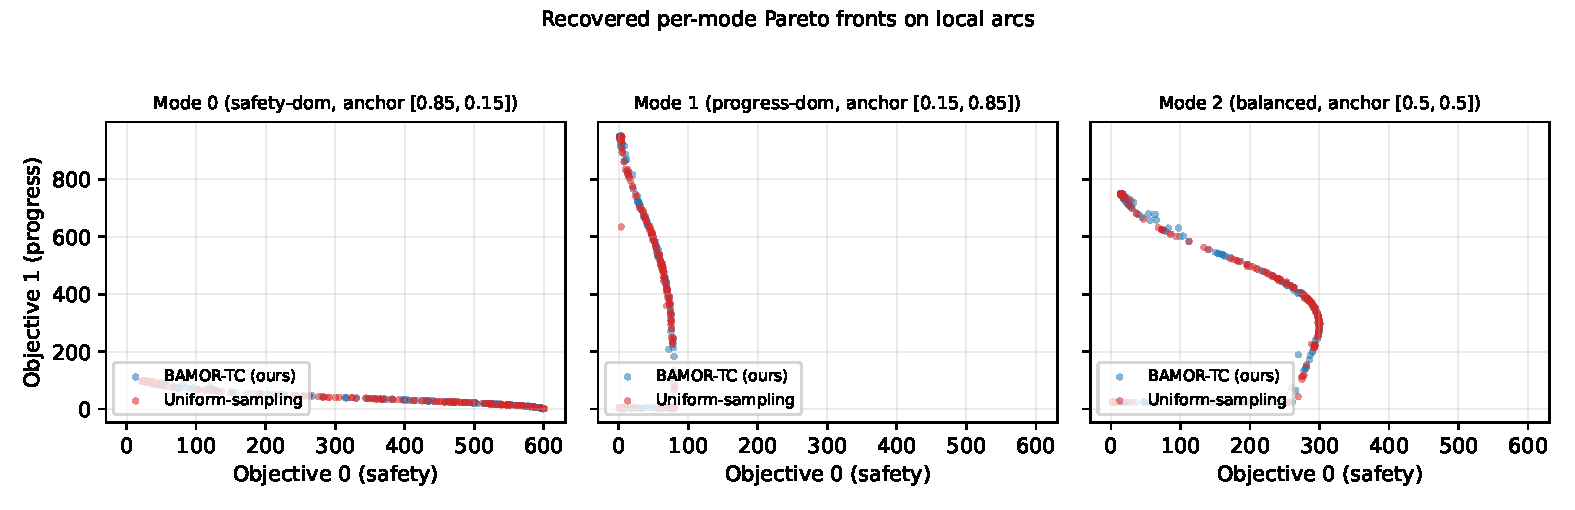
\includegraphics[width=0.98\linewidth]{fig_pareto_permode.pdf}
\caption{Per-mode Pareto fronts recovered by BAMOR-TC and Uniform, pooled across seeds and weights in the evaluation grid. Mode~0's front is a near-horizontal arc (progress capped), Mode~1's is near-vertical (safety capped), and Mode~2 is a full elbow. Both methods recover the same mode-wise geometry, while Uniform shows more low-return scatter in several panels.}
\label{fig:pareto_permode}
\end{figure}

Fig.~\ref{fig:pareto_permode} illustrates the different return geometries of the three synthetic modes. These are separate mode-conditioned fronts; their union is not the Pareto front of a single common evaluation task.  The substrate caps in Modes~0 and~1 appear as near-horizontal and near-vertical arcs respectively.  Uniform produces the same general shape but with more low-return/off-arc scatter in several panels.  BAMOR-TC's target-cone sampler targets each arc directly.

% ── 6.5 Training dynamics ───────────────────────────────────────────────────
\subsection{Training dynamics and stability}

\begin{figure}[t]
\centering
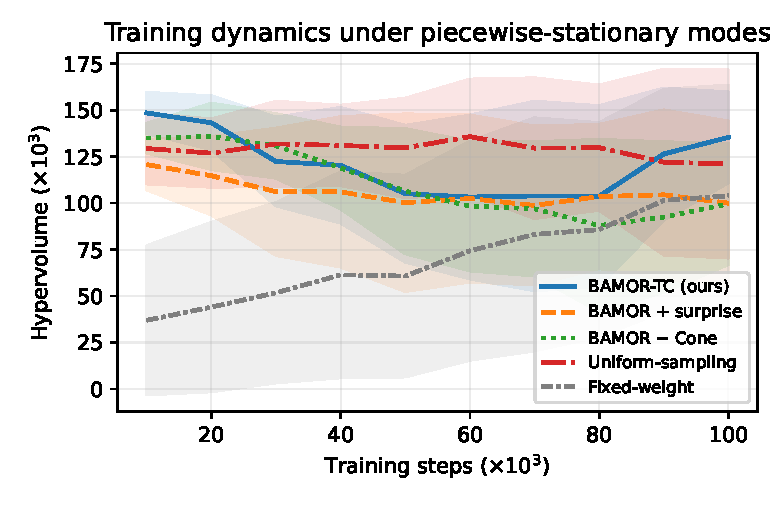
\includegraphics[width=0.72\linewidth]{fig_training_curves_v2.pdf}
\caption{Overall HV during training.  Shaded bands are $\pm1\sigma$ across 20 seeds.  BAMOR-TC (blue) starts high, loses ground in the middle training window, then recovers after $80$k steps and finishes with the highest mean and a tighter final band than Uniform.  Uniform (red) is steadier through the middle but ends lower.  BAMOR $+$ surprise (orange) and BAMOR $-$ Cone (green) finish well below BAMOR-TC.  Fixed-weight (grey) improves late but remains high-variance.}
\label{fig:training_curves}
\end{figure}

Fig.~\ref{fig:training_curves} shows HV trajectories during training.  Two qualitative patterns stand out.  First, BAMOR-TC is not a pointwise-dominant training curve: it starts high, falls below Uniform in the middle window, and then recovers sharply by the final evaluations.  The defensible claim is final HV and lower final variance, not monotone dominance at every checkpoint.  Second, both adaptive ablations have lower final sample means than BAMOR-TC. The paired synthetic comparison and ablation limitations above restrict a causal interpretation of these curves.

% ── 6.6 Continuous-control stress test ─────────────────────────────────────

\clearpage
\subsection{Historical Continuous-Control Comparison}
\label{app:historical_continuous}

The original 20-seed, 50k-step v23 study used 19 BAMOR actor snapshots but
one CAPQL actor. Its overall evaluator advanced a persistent mode schedule
across episodes, weights and actors. Changing the number or order of candidates
therefore changed evaluation conditions as well as the evaluated policy set.
Table~\ref{tab:mujoco_3d_policy_set} is retained as a historical record and is
not used in the matched-comparison conclusions.

\begin{table}[t]
\centering\footnotesize
\caption{Historical exploratory continuous-control results, retained with their original metric. HV is in billions (B). BAMOR-v23 and v22 use 19 actor snapshots; CAPQL uses its final actor. The overall evaluator advances a persistent mode schedule between candidates, so this is not an archive-matched or common-distribution comparison. Bottom20 is the mean of the lowest 20\% of seeds; wins and two-sided Wilcoxon $p$ values describe this historical metric only. HalfCheetah has two objectives; Ant and Hopper have three.}
\label{tab:mujoco_3d_policy_set}
\begin{tabular}{llrrrrcc}
\toprule
Env & Method & Mean & Median & Bottom20 & Min & Wins & $p$ \\
\midrule
\multirow{4}{*}{HalfCheetah}
& Uniform & 0.001 & 0.000 & 0.000 & 0.000 & 20/20 & $<10^{-4}$ \\
& CAPQL & 0.004 & 0.003 & 0.001 & 0.000 & 14/20 & 0.0328 \\
& BAMOR-v22 & 0.006 & 0.006 & 0.003 & 0.002 & 11/20 & 0.5706 \\
& \textbf{BAMOR-v23} & \textbf{0.006} & 0.005 & \textbf{0.004} & \textbf{0.003} & -- & -- \\
\midrule
\multirow{6}{*}{Ant}
& Uniform & 12.671 & 9.460 & 2.584 & 2.185 & 20/20 & $<10^{-4}$ \\
& CAPQL & 10.137 & 4.466 & 2.665 & 2.292 & 20/20 & $<10^{-4}$ \\
& BAMOR & 13.769 & 16.661 & 2.931 & 2.381 & 20/20 & $<10^{-4}$ \\
& v5 MoE-template & 12.312 & 11.405 & 2.487 & 2.266 & 20/20 & $<10^{-4}$ \\
& v6 shared-head MoE & 13.441 & 16.136 & 2.587 & 2.185 & 20/20 & $<10^{-4}$ \\
& \textbf{BAMOR-v23} & \textbf{40.899} & \textbf{40.495} & \textbf{36.918} & \textbf{34.123} & -- & -- \\
\midrule
\multirow{6}{*}{Hopper}
& Uniform & 1.500 & 1.618 & 0.026 & 0.017 & 18/20 & 0.0001 \\
& CAPQL & 4.335 & 2.835 & 1.325 & 0.487 & 14/20 & 0.0973 \\
& BAMOR & 2.287 & 1.610 & 0.024 & 0.016 & 16/20 & 0.0014 \\
& v5 MoE-template & 2.412 & 2.368 & 0.408 & 0.027 & 17/20 & 0.0002 \\
& v6 shared-head MoE & 2.406 & 2.347 & 0.459 & 0.018 & 20/20 & $<10^{-4}$ \\
& \textbf{BAMOR-v23} & \textbf{6.193} & \textbf{4.818} & \textbf{2.851} & \textbf{2.804} & -- & -- \\
\bottomrule
\end{tabular}
\end{table}


The historical locked-mode diagnostic used restricted preference grids and
unmatched episode resets. Mean mode-wise archive/final HV, v23 versus CAPQL,
was 3.032M/2.221M on HalfCheetah, 2.096B/1.838B on Ant and 3.357B/1.914B
on Hopper. Even there, HalfCheetah mode 3 favored CAPQL, 1.653M versus 0.827M.
The current main-text comparisons replace these settings with common locked
modes, full-simplex grids and episode reset seeds.
\FloatBarrier


\end{document}
